\section{Alternative Evaluation Methodologies} \label{appendix:amethodology}

\noindent In the main paper, we develop and document the results from two methodologies to account for treatment substitution in the first phase of ABC/CARE. The objective of each method is to estimate the average treatment effect of ABC/CARE, holding fixed take-up of alternative preschool by the control groups. We want to construct a scenario in which the subjects in the control group do not attend alternative preschool. This allows us to evaluate center-based childcare relative to a counterfactual scenario in which subjects stay at home.\\

\noindent This section presents alternative methodologies to evaluate the first-phase treatment. Throughout the rest of this section, we refer to treatment in either ABC/CARE generically as center-based childcare, as we discard the family education treatment group of CARE---as in the main paper, the control group consists of the control groups in both ABC and CARE. We refer to take-up of treatment substitution as enrollment into alternative preschool. As in our main methodology, we choose the control sets to account for background variables using the method in Appendix~\ref{appendix:results}.\\

\noindent To illustrate the alternative methodologies, we present results for a small set of outcomes. First, we consider a time series of IQ scores. Second, we present results for three long-term outcomes: years of education, employment, and labor income. Both IQ scores and the chosen long-term outcomes follow predictable patterns and are straightforward to interpret. These characteristics allow us to evaluate the sensitivity of the estimated treatment effects using the different strategies.\\

\noindent Let the discrete choice to enroll in alternative preschool, $P$, be defined as $P=\mathbf{1}\left[V>0\right]$ which is an indicator equal to 1 when the subject is enrolled. Let $Q$ be the number of months in alternative preschool. $\mathbf{X}$ is a vector of observed individual- or household-level characteristics. $P$ and $Q$ are zero for participants of the treatment group. In this section, we allow for the take-up of the program to be imperfectly given by the randomization. Let $D$ be take-up of the ABC/CARE program.

\subsection{Instrumental Variables}

\noindent The first alternative method we present is based on a standard, linear instrumental variable framework.

\subsubsection{Model and Conditions}

\noindent Consider the following equation for an outcome $Y$:


\begin{equation}
Y = \alpha^D D + \alpha^Q Q + \mathbf{X} \beta + \varepsilon,
\label{eq:ivnot}
\end{equation}

\noindent where $D$ and $Q$ are endogenous. Selection into treatment or alternative preschool is likely correlated with characteristics not observed when estimating the coefficients characterizing the outcome equation, i.e., $Cov(D,\varepsilon) \neq 0$ and $Cov(Q,\varepsilon) \neq 0$. Estimating the coefficients in \eqref{eq:ivnot} by OLS yields inconsistent estimates.\\

\noindent A standard solution is to introduce a vector of instrumental variables, $\mathbf{Z}$, satisfying two conditions: (i) the matrix $\Pi$ of the coefficients in the population regression of $D$ and $Q$ on $\mathbf{Z}$ is full rank; and (ii) $\mathbf{Z}$ is uncorrelated with $\varepsilon$.


\subsubsection{Instrumental Variables in Practice}

\noindent To identify the coefficients in \eqref{eq:ivnot} using an instrumental variable strategy we need at least two instruments. We use randomization into ABC/CARE treatment as an instrument, denoted as an indicator, $R$. We then consider up to three other instruments.

\begin{enumerate}[(i)]
\item \textit{Season of subject's birth}. This variable is coded as an indicator for being born in the fall (born between June and November). If preschools accepted children primarily in the fall, then children born in the fall could enter preschool when they were younger. Although there is evidence in the economics literature that being born during specific times in the year can influence a child's outcomes, the main channel for this effect seems to be the disproportionate selection into season of birth by high-income mothers \citep{Buckles-Hungerman_2013_RES}. Given that the mothers were very young and disadvantaged in the ABC/CARE sample, we assume that a negligible proportion of them selected their quarter of birth.

\item \textit{Presence of a grandmother in the county}. We hypothesize that the grandmothers of the subjects, who in this sample are relatively young and still working, could help the study mothers take care of their children. We assume that the mothers would have less influence over the presence of a grandmother in the county as opposed to the presence of a grandmother living in the home. We also assume that the grandmothers do not affect the subjects differently than any other avenue of informal care, such as care from a neighbor. In practice, the presence of a grandmother has a positive effect on preschool attendance, which could indicate that they helped take the subject to preschool. This variable is only available for ABC.

\item \textit{Number of relatives living in the household apart from the mother, subject, siblings, and male partner}. We assume that the relatives could take care of the subject while the mother was at work or in school, but that they do not affect the subjects differently than any other avenue of informal care. In practice, having additional relatives living at home decreases the probability that the subject goes into preschool.
\end{enumerate}

\subsubsection{Sets of Instruments}
\noindent We consider three combinations of the instruments.  All of them include randomization into center-based treatments and birth in the fall. All of them include at least one variable representing access to informal care from relatives. The sets are the following:
\begin{enumerate}[(i)]
\item Randomization, Born in the Fall, Grandmother in County, Number of Relatives at Home
\item Randomization, Born in the Fall, Grandmother in County
\item Randomization, Born in the Fall, Number of Relatives at Home
\end{enumerate}

\subsubsection{Specifications for the Instruments}
\noindent We test various specifications in which we allow for interactions of the potential instruments with the first-phase randomization indicator. In particular, we test three specifications for our instruments:

\begin{enumerate}[(i)]
\item Instruments measured in levels: $ \left( R,\mathbf{Z} \right) $.
\item\label{interact} Instruments measured in levels and interactions of treatment with the instruments and the controls: $ \left(R,\mathbf{Z},\mathbf{Z}R,\mathbf{X}R \right)$.
\item\label{inverse} Interactions of the instruments and the controls with an indicator for being randomized into the control group: $\left( R, \mathbf{X} \left( 1-R \right), \mathbf{Z} \left( 1-R \right) \right)$.
\end{enumerate}

\noindent In practice, the specification in \eqref{inverse} is the most stable across outcomes. This makes economic sense because the instruments are less likely to affect the participants of the treatment group, given that almost all the treatment families comply to the first-phase randomization protocol.

\subsubsection{Functional Forms of Enrollment in Alternative Preschool}

\noindent We use a different parameterization of enrollment into alternative preschool in \eqref{eq:ivnot}:

\begin{enumerate}[(i)]
\item The number of months in alternative preschool, $Q$.
\item An indicator for take-up of alternative preschool, $P$.
\item The $\log$ of months in alternative preschool, $\log Q$.
\end{enumerate}

\subsection{Results}

\noindent In this section, we present the results of the instrumental variable approach. We discuss the estimates of the coefficient for $D$ in \eqref{eq:ivnot}, while accounting for endogenous take-up of alternative preschool. The results are roughly stable for all presented outcomes: the effect considering the take-up of alternative preschool in the control group is much stronger than the intent-to-treat effect (the mean difference between the treatment and control groups). At ages 15 and 21, the effects on IQ scores are close to zero.

\subsubsection{Main Specification}

\noindent Our main specification uses three instruments: randomization into center-based childcare in ABC/CARE, the presence of a grandmother in the county, and being born in the fall. We interact the latter two instrument with an indicator for being randomized into the control group ($1-R$). The endogenous variables are $D$ and $Q$.\\

\noindent Figure \ref{fig:main_iv1} and Figure~\ref{fig:mainiv2} display the estimates of the coefficient of $D$. That is, the effect of attending the ABC/CARE treatment, fixing take-up of alternative preschool. The results indicate the following: (i) the effects are stronger compared to those in the main paper, even compared to those in the main paper that fix subjects to no preschool alternatives; (ii) the estimates are less stable across ages compared to those in the main paper. For example, while the effects on IQ scores from ages 0 to 5 average around 14 points in the main paper, they average 20 points using this specification of instrumental variables.

\begin{figure}[H]
		\caption{Effect of Center-based Childcare on IQ Scores, Accounting for Endogenous Take-up of Alternative Preschool Using Instrumental Variables} \label{fig:main_iv1}
		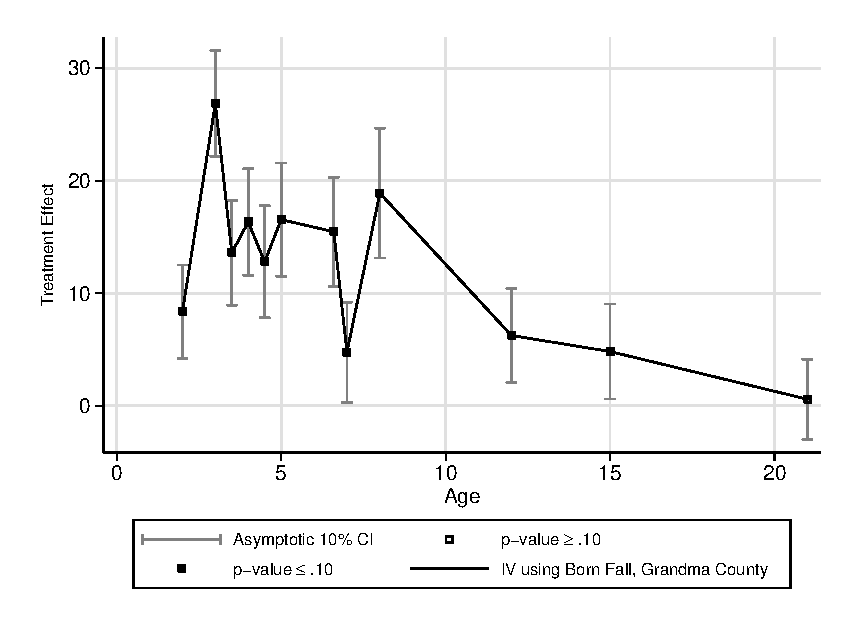
\includegraphics[width=.8\columnwidth]{output/appendixplots/main_iv_te.eps}
\floatfoot{
\footnotesize
\noindent Note: This plot presents the parameter associated with $D$ from a regression of $Y$ on $D$, $Q$, and $\mathbf{X}$, using $R$ and $\mathbf{Z}(1-R)$ as instruments. The outcomes ($Y$) are IQ tests at different ages, with a national standard deviation of 15 and a mean of 100. $\mathbf{X}$ includes a set of controls selected from all available baseline controls to maximize explanatory power across all outcomes tested in the paper: gender of the subject, mother's IQ score, High-risk Index, and Apgar Score at 1 minute. The confidence intervals are calculated at the 10\% significance level.}
\end{figure}

\begin{figure}[H]
		\caption{Effect of Center-based Childcare on Labor Market Outcomes, Accounting for Endogenous Take-up of Alternative Preschool Using Instrumental Variables} \label{fig:mainiv2}
		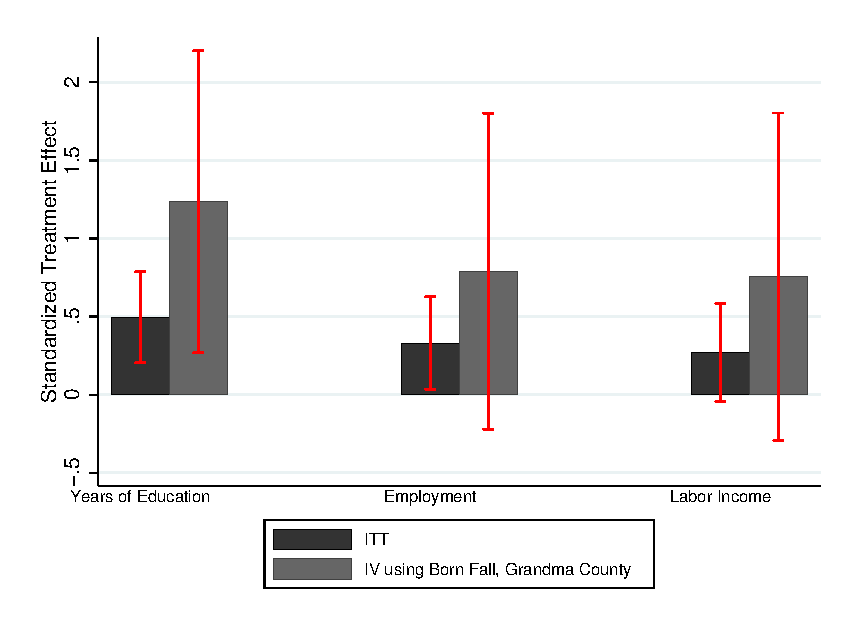
\includegraphics[width=.8\columnwidth]{output/appendixplots/main_iv_other.eps}
\floatfoot{
\footnotesize
\noindent Note: This plot presents the parameter associated with $D$ from a regression of $Y$ on $D$, $Q$, and $\mathbf{X}$, using $R$ and $\mathbf{Z}(1-R)$ as instruments. The outcomes ($Y$) are different adult outcomes labeled in the horizontal axis. $\mathbf{X}$ includes a set of controls selected from all available baseline controls to maximize explanatory power across all outcomes tested in the paper: gender of the subject, mother's IQ score, High-risk Index, and Apgar Score at 1 minute. The confidence intervals are calculated at the 10\% significance level.}
\end{figure}

\subsubsection{Varying the Sets of Instruments}

\noindent Figure \ref{fig:ins_inter_Q_iv1} and Figure \ref{fig:ins_inter_Q_iv2} explore the sensitivity of the estimates to different sets of instruments. The pattern of results indicates that the method is generally robust to the three sets of instrumental variables that we consider.

\begin{figure}[H]
		\caption{Effect of Center-based Childcare on IQ Scores, Accounting for Endogenous Take-up of Alternative Preschool Using Various Instrumental Variables} \label{fig:ins_inter_Q_iv1}
		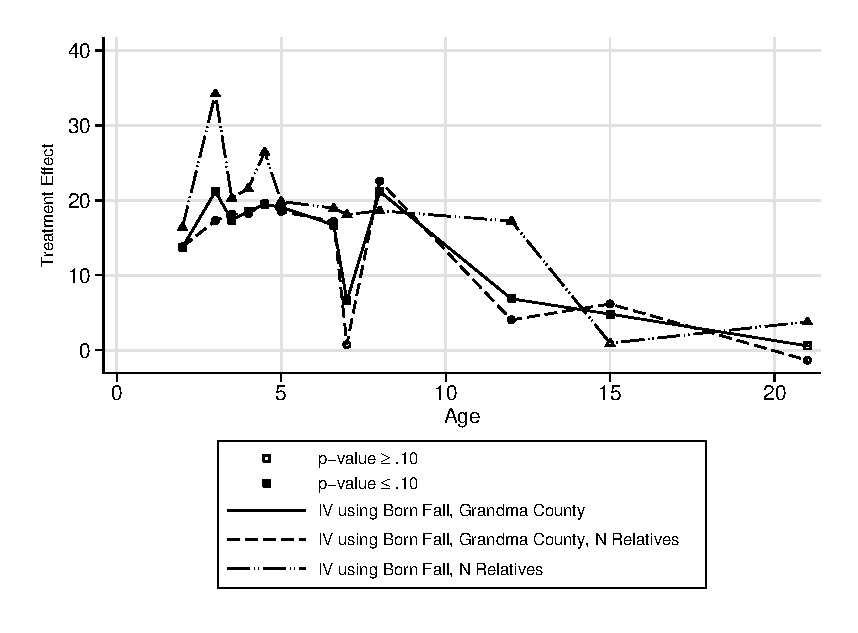
\includegraphics[width=.8\columnwidth]{output/appendixplots/ins_inter_Q_iv_te.eps}
\floatfoot{
\footnotesize
\noindent Note: This plot presents the parameter associated with $D$ from a regression of $Y$ on $D$, $Q$, and $\mathbf{X}$, using $R$ and $\mathbf{Z}(1-R)$ as instruments. The outcomes ($Y$) are IQ scores at different ages, with a national standard deviation of 15 and a mean of 100. $\mathbf{X}$ includes a set of controls selected from all available baseline controls to maximize explanatory power across all outcomes tested in the paper: gender of the subject, mother's IQ score, High-risk Index, and Apgar Score at 1 minute. The confidence intervals are calculated at the 10\% significance level.}
\end{figure}

\begin{figure}[H]
		\caption{Effect of Center-based Childcare on Labor Market Outcomes, Accounting for Endogenous Take-up of Alternative Preschool Using Various Instrumental Variables} \label{fig:ins_inter_Q_iv2}
		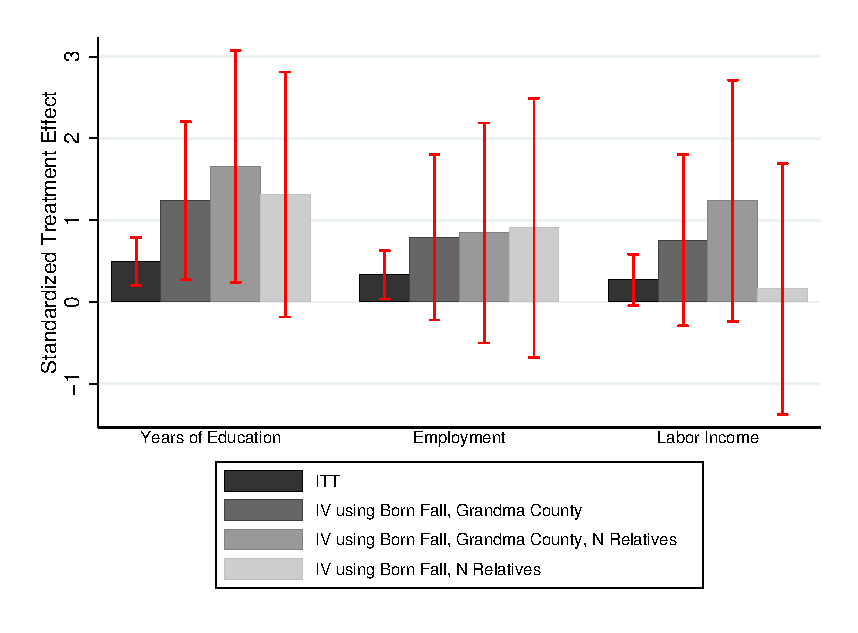
\includegraphics[width=.8\columnwidth]{output/appendixplots/ins_inter_Q_iv_other.eps}
\floatfoot{
\footnotesize
\noindent Note: This plot presents the parameter associated with $D$ from a regression of $Y$ on $D$, $Q$, and $\mathbf{X}$, using $R$ and $\mathbf{Z}(1-R)$ as instruments. The outcomes ($Y$) are different adult outcomes labeled in the horizontal axis. $\mathbf{X}$ includes a set of controls selected from all available baseline controls to maximize explanatory power across all outcomes tested in the paper: gender of the subject, mother's IQ score, High-risk Index, and Apgar Score at 1 minute. The confidence intervals are calculated at the 10\% significance level.}
\end{figure}

\subsubsection{Varying the Specification of the Instruments}

\noindent We now present an exercise to evaluate the sensitivity of the results to different specifications of the instrumental variables. First, Figure~\ref{fig:nointer_Q_iv} and Figure~\ref{fig:nointer_Q_other} present the results using the set of instruments that are not interacted with an indicator for randomization into the control group ($1-R$). Figure~\ref{fig:inter_Q_iv} and Figure~\ref{fig:inter_Q_other} present results not only interacting the instruments but also interacting the observed characteristics we control for. In both exercises, we use $Q$ as the endogenous variable, along with $D$.\\

\noindent The results follow the same patterns as before, although they change when the instruments are not interacted. This makes economic sense because the interacted instruments better represent the economic intuition we offer before: the instruments other than $R$ are more likely to shift the decisions of the families of the control-group subjects compared to those of the treatment-group subjects.

\begin{figure}[H]
		\caption{Effect of Center-based Childcare on IQ Scores, Accounting for Endogenous Take-up of Alternative Preschool Using Various Instrumental Variables Specifications} \label{fig:nointer_Q_iv}
		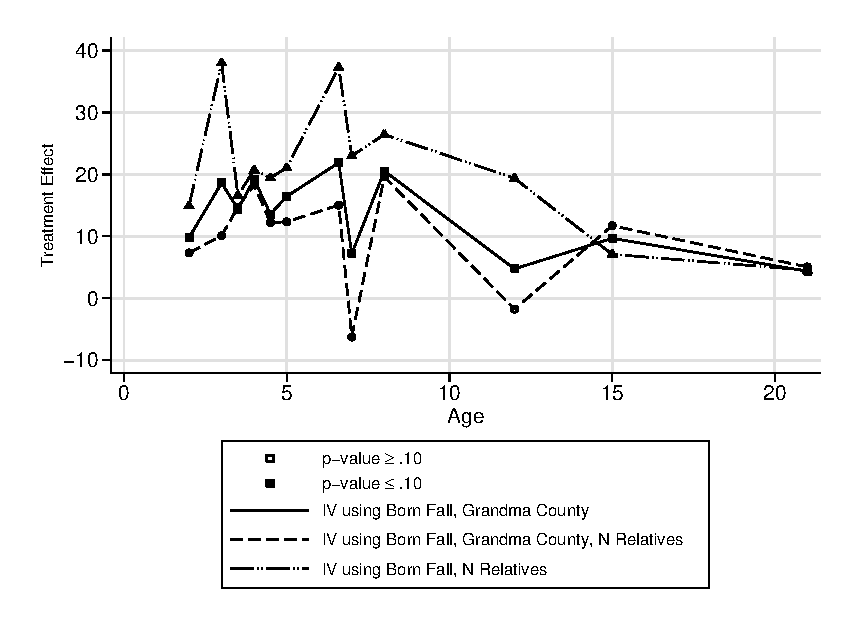
\includegraphics[width=.8\columnwidth]{output/appendixplots/nointer_Q_iv_te.eps}
\floatfoot{
\footnotesize
\noindent Note: This plot presents the parameter associated with $D$ from a regression of $Y$ on $D$, $Q$, and $\mathbf{X}$, using $R$ and $\mathbf{Z}$ as instruments. $Y$ is different IQ tests, with a national standard deviation of 15 and a mean of 100. $\mathbf{X}$ includes a set of controls selected from all available baseline controls to maximize explanatory power across all outcomes tested in the paper: gender of the subject, mother's IQ, High-risk Index, and Apgar Score at 1 minute. The confidence intervals are calculated at the 10\% significance level.}
\end{figure}

\begin{figure}[H]
		\caption{Effect of Center-based Childcare on Labor Market Outcomes, Accounting for Endogenous Take-up of Alternative Preschool Using Various Instrumental Variables Specifications} \label{fig:nointer_Q_other}
		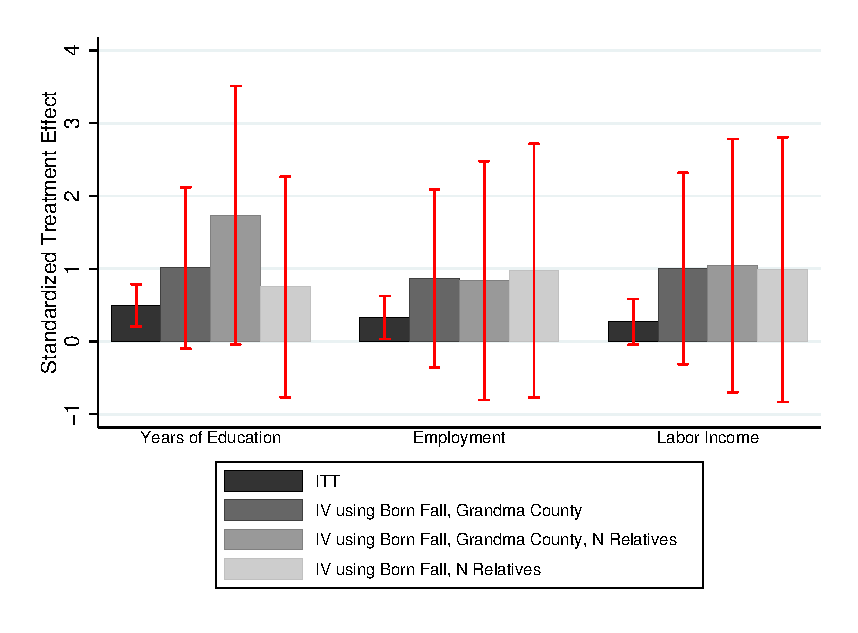
\includegraphics[width=.8\columnwidth]{output/appendixplots/nointer_Q_iv_other.eps}
\floatfoot{
\footnotesize
\noindent Note: This plot presents the parameter associated with $D$ from a regression of $Y$ on $D$, $Q$, and $\mathbf{X}$, using $R$ and $\mathbf{Z}$ as instruments. The outcomes ($Y$) are different adult outcomes labeled in the horizontal axis. $\mathbf{X}$ includes a set of controls selected from all available baseline controls to maximize explanatory power across all outcomes tested in the paper: gender of the subject, mother's IQ score, High-risk Index, and Apgar Score at 1 minute. The confidence intervals are calculated at the 10\% significance level.}
\end{figure}

\begin{figure}[H]
		\caption{Effect of Center-based Childcare on IQ Scores, Accounting for Endogenous Take-up of Alternative Preschool Using Various Instrumental Variables Specifications} \label{fig:inter_Q_iv}
		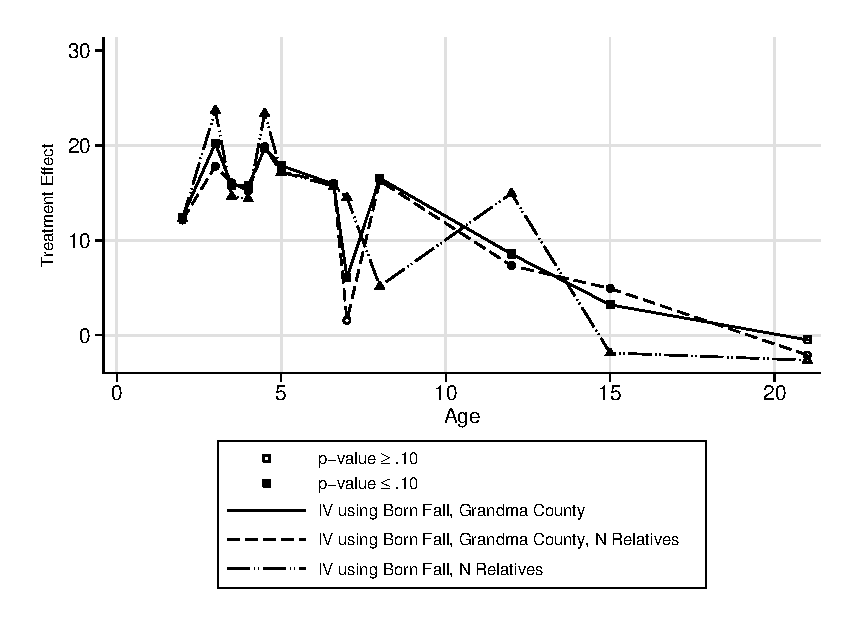
\includegraphics[width=.8\columnwidth]{output/appendixplots/inter_Q_iv_te.eps}
\floatfoot{
\footnotesize
\noindent Note: This plot presents the parameter associated with $D$ from a regression of $Y$ on $D$, $Q$ ,and $\mathbf{X}$, using $R$, $\mathbf{X}(1 - R)$ and $\mathbf{Z}(1 - R)$ as instruments. The outcomes ($Y$) are IQ scores at different ages, with a national standard deviation of 15 and a mean of 100. $\mathbf{X}$ includes a set of controls selected from all available baseline controls to maximize explanatory power across all outcomes tested in the paper: gender of the subject, mother's IQ score, High-risk Index, and Apgar Score at 1 minute. The confidence intervals are calculated at the 10\% significance level.}
\end{figure}

\begin{figure}[H]
		\caption{Effect of Center-based Childcare on Labor Market Outcomes, Accounting for Endogenous Take-up of Alternative Preschool Using Various Instrumental Variables Specifications} \label{fig:inter_Q_other}
		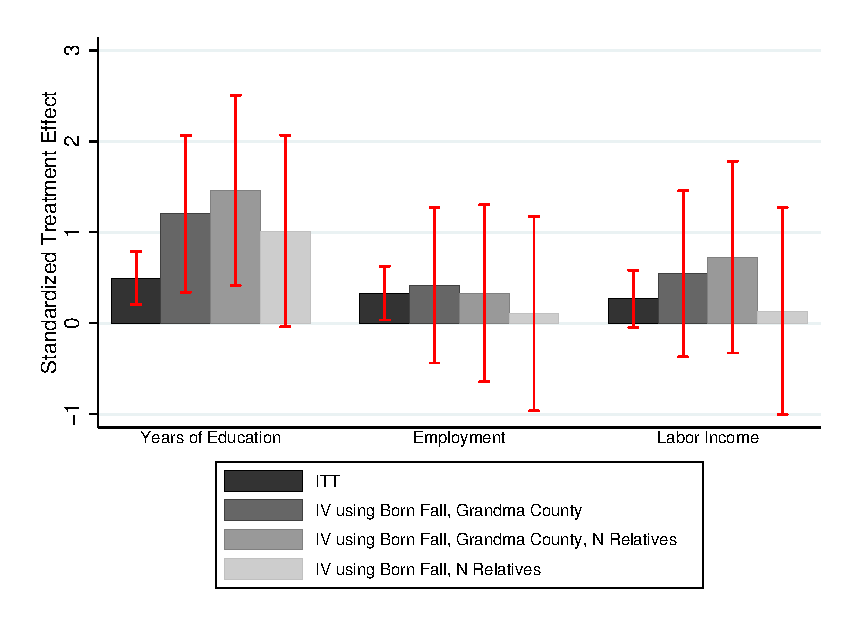
\includegraphics[width=.8\columnwidth]{output/appendixplots/inter_Q_iv_other.eps}
\floatfoot{
\footnotesize
\noindent Note: This plot presents the parameter associated with $D$ from a regression of $Y$ on $D$, $Q$, and $\mathbf{X}$, using $R$, $\mathbf{X}(1 - R)$ and $\mathbf{Z}(1 - R$) as instruments. The outcomes ($Y$) are different adult outcomes labeled in the horizontal axis. $\mathbf{X}$ includes a set of controls selected from all available baseline controls to maximize explanatory power across all outcomes tested in the paper: gender of the subject, mother's IQ score, High-risk Index, and Apgar Score at 1 minute. The confidence intervals are calculated at the 10\% significance level.}
\end{figure}

\subsubsection{Varying the Parameterization of Alternative Preschool Take-up}

\noindent Now, we explore the sensitivity to the specification of $Q$ in \eqref{eq:ivnot}. We consider two alternatives. First, we use an indicator of take-up of alternative preschool, $P$ (Figure~\ref{fig:ins_inter_P_iv} and Figure~\ref{fig:ins_inter_P_other}). Second, we take the $\log$ of $Q$ (Figure~\ref{fig:ins_inter_LogQ_iv} and Figure~\ref{fig:ins_inter_LogQ_other}).

\begin{figure}[H]
		\caption{Effect of Center-based Childcare on IQ Scores, Accounting for an Endogenous Indicator of Take-up of Alternative Preschool} \label{fig:ins_inter_P_iv}
		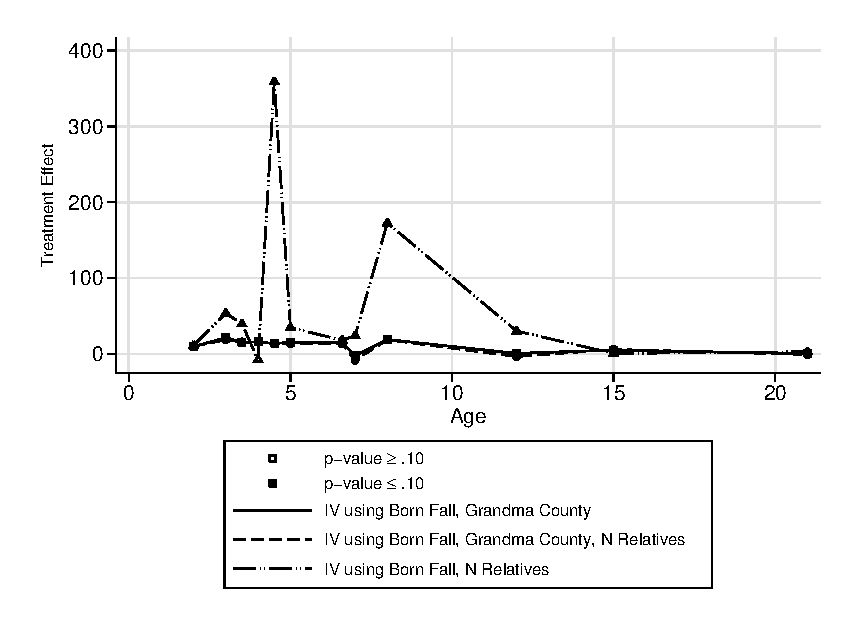
\includegraphics[width=.8\columnwidth]{output/appendixplots/ins_inter_P_iv_te.eps}
\floatfoot{
\footnotesize
\noindent Note: This plot presents the parameter associated with $D$ from a regression of $Y$ on $D$, $P$, and $\mathbf{X}$, using $R$, $\mathbf{Z}(1 - R)$ as instruments. The outcomes ($Y$) are IQ scores at different ages, with a national standard deviation of 15 and a mean of 100. $\mathbf{X}$ includes a set of controls selected from all available baseline controls to maximize explanatory power across all outcomes tested in the paper: gender of the subject, mother's IQ score, High-risk Index, and Apgar Score at 1 minute. The confidence intervals are calculated at the 10\% significance level.}
\end{figure}

\begin{figure}[H]
		\caption{Effect of Center-based Childcare on Labor Market Outcomes, Accounting for an Endogenous Indicator of Take-up of Alternative Preschool} \label{fig:ins_inter_P_other}
		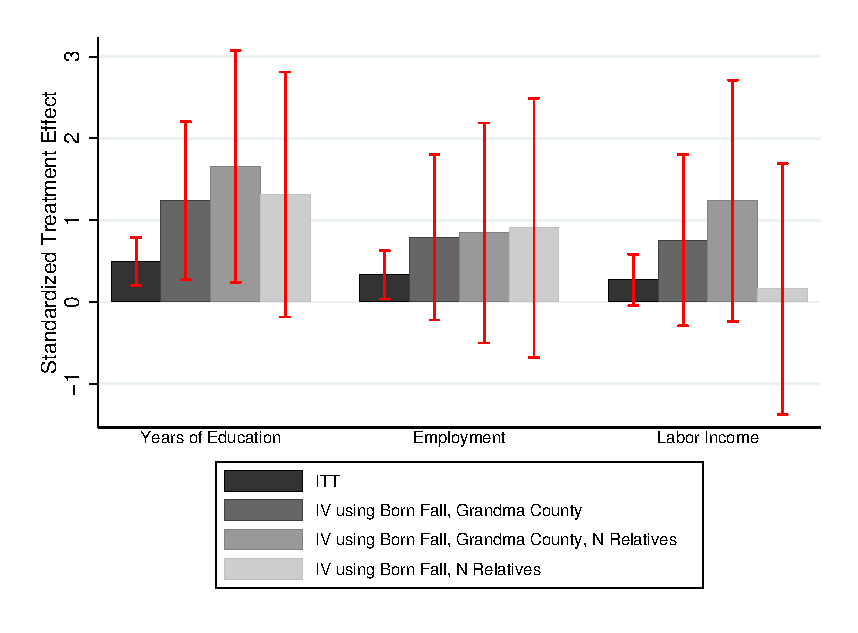
\includegraphics[width=.8\columnwidth]{output/appendixplots/ins_inter_P_iv_other.eps}
\floatfoot{
\footnotesize
\noindent Note: This plot presents the parameter associated to $D$ from a regression of $Y$ on $D$, $P$, and $\mathbf{X}$, using $R$, $\mathbf{Z}(1 - R$) as instruments. The outcomes ($Y$) are different relevant adult outcomes labeled in the horizontal axis. $\mathbf{X}$ includes a set of controls selected from all available baseline controls to maximize explanatory power across all outcomes tested in the paper: gender of the subject, mother's IQ score, High-risk Index, and Apgar Score at 1 minute. The confidence intervals are calculated at the 10\% significance level.}
\end{figure}

\begin{figure}[H]
		\caption{Effect of Center-based Childcare on IQ Scores, Accounting for Endogenous (log) Months of Take-up of Alternative Preschool} \label{fig:ins_inter_LogQ_iv}
		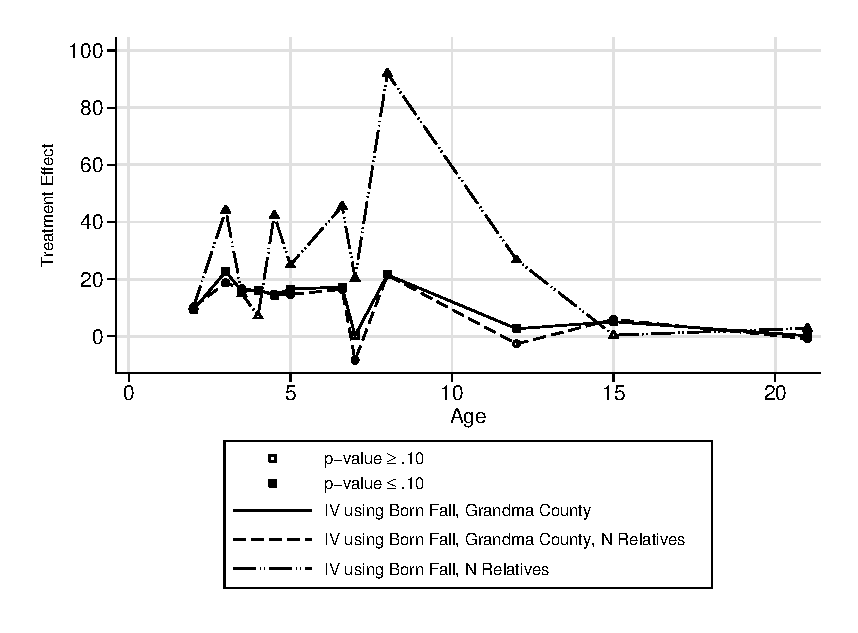
\includegraphics[width=.8\columnwidth]{output/appendixplots/ins_inter_logQ_iv_te.eps}
\floatfoot{
\footnotesize
\noindent Note: This plot presents the parameter associated with $D$ from a regression of $Y$ on $D$, $\log Q$, and $\mathbf{X}$, using $R$, $\mathbf{Z}(1 - R)$ as instruments. The outcomes ($Y$) are IQ scores at different ages, with a national standard deviation of 15 and a mean of 100. $\mathbf{X}$ includes a set of controls selected from all available baseline controls to maximize explanatory power across all outcomes tested in the paper: gender of the subject, mother's IQ score, High-risk Index, and Apgar Score at 1 minute. The confidence intervals are calculated at the 10\% significance level.}
\end{figure}

\begin{figure}[H]
		\caption{Effect of Center-based Childcare on Labor Market Outcomes, Accounting for Endogenous (log) Months of Take-up of Alternative Preschool} \label{fig:ins_inter_LogQ_other}
		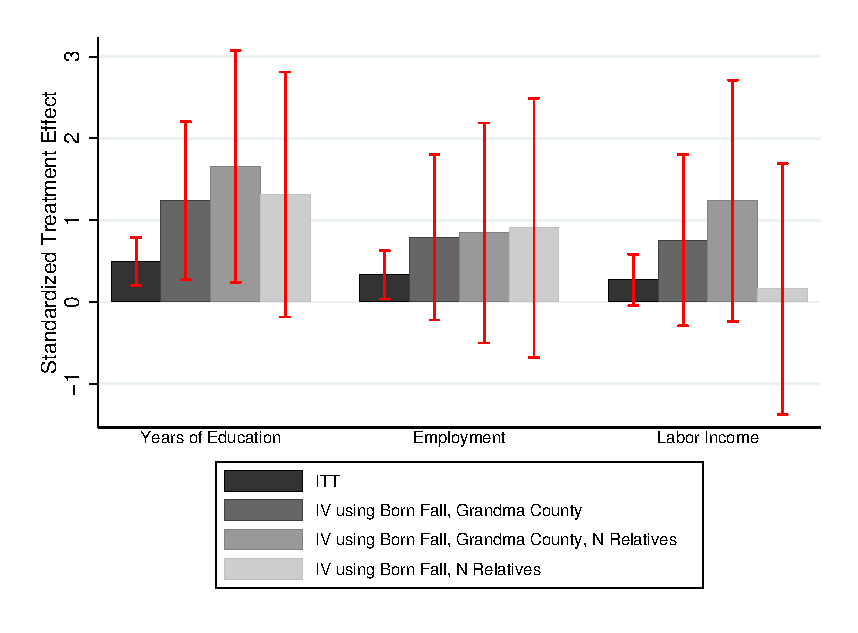
\includegraphics[width=.8\columnwidth]{output/appendixplots/ins_inter_logQ_iv_other.eps}
\floatfoot{
\footnotesize
\noindent Note: This plot presents the parameter associated with $D$ from a regression of $Y$ on $D$, $\log Q$, and $\mathbf{X}$, using $R$, $\mathbf{Z}(1 - R$) as instruments. The outcomes ($Y$) are different adult outcomes labeled in the horizontal axis. $\mathbf{X}$ includes a set of controls selected from all available baseline controls to maximize explanatory power across all outcomes tested in the paper: gender of the subject, mother's IQ score, High-risk Index, and Apgar Score at 1 minute. The confidence intervals are calculated at the 10\% significance level.}
\end{figure}


\subsection{Control Functions}

\noindent We now consider a control function approach. With control functions, the objective is also to simultaneously account for take-up of center-based childcare and alternative preschool.

\subsubsection{Setup}

\noindent The method we propose is an application of the selection correction in \citet{Heckman_1979_Econometrica}. We model the selection into both endogenous variables of interest, center-based childcare and alternative preschool. The method involves three equations: (i) the outcome equation; (ii) the probability of participating in center-based childcare; (iii) a linear equation describing the number of months enrolled in preschool alternatives.\\

\noindent Let $Y^{0}$ be the counterfactual outcome of subject $i$ when not participating in center-based childcare. Similarly, let $Y^{1}$ be her potential outcome if she participates. We model the outcome as:

\begin{eqnarray}
Y^1 &=& \alpha^1+\mathbf{X} \mathbf{\beta}                 +\varepsilon^1 \nonumber  \\
Y^0 &=& \alpha^0+\mathbf{X} \mathbf{\beta} + \alpha^Q Q+\varepsilon^0.  \label{eq:potout}
\end{eqnarray}

\noindent The equation describing participation in center-based childcare is:

\begin{equation}
D = \left\{
        \begin{array}{ll}
        	0 &\text{if } D^* \leq  0 \\
            1 &\text{if } D^* > 0, \label{eq:sel1}
        \end{array}
    \right.
\end{equation}

\noindent where we interpret $D^*$ as a latent continuous variable representing the household's interest in sending the subject to treatment. We write

\begin{equation}
D^{*} = \mathbf{W} \gamma^{D} + \varepsilon^{D}, \label{eq:probitD}
\end{equation}

\noindent where $\mathbf{W}$ is a vector that includes $\mathbf{X}$ and $R$ and can include variables that shift the decision to enroll subjects into ABC/CARE without shifting the counterfactual outcome of interest, $Y^{d}$. \\

\noindent We model the selection into months of alternative preschool as a linear equation with fixed coefficients, assuming homogeneous treatment effects:

\begin{equation}
Q = \mathbf{W} \gamma^{Q} + \varepsilon^{Q}, \label{eq:selq}
\end{equation}

\noindent In general, the unobserved variables in each of these equations are correlated. We assume that they are distributed as follows:

\begin{equation}
        \left[ \begin{array}{l}
        	 \varepsilon^1 \\
            \varepsilon^0 \\
            \varepsilon^D
        \end{array} \right]  \sim \mathcal{N} \left[ \left( \begin{array}{l}
        	 0 \\
           0 \\
           0
        \end{array} \ \right),
                \left( \begin{array}{llll}
        	 \sigma_{1}^2 & \sigma_{1,0} & \sigma_{1,D}   \\
             \sigma_{1,0} & \sigma_{0}^2 & \sigma_{0,D}   \\
             \sigma_{1,D} & \sigma_{0,D} & 1
        \end{array} \right) \right],  \label{eq:udist}
\end{equation}

\noindent where we normalize $\var \left( \varepsilon^D \right) =1$.\\

\noindent Further, we assume that
\begin{equation}
\mathbb{E}\left[\varepsilon^0|D=0,\mathbf{W},\varepsilon^{Q},Q=q\right]=\sigma^{0,Q}\varepsilon^{Q}+\mathbb{E}\left[\varepsilon^0|D=0,\mathbf{W}\right].
\label{eq:E[epsilon0]}
\end{equation}

\subsubsection{Identification}

\noindent The following steps identify the parameters of interest. First, we estimate the parameters characterizing the decision to enroll the subject in center-based childcare. We exploit the assumption that $\varepsilon^D \sim \mathcal{N} \left( 0, 1 \right)$ in \eqref{eq:udist} and estimate the parameters in \eqref{eq:probitD} using a probit model.\\

\noindent Second, we approximate the unobserved term relevant to the choice of $Q$. We take the coefficients in \eqref{eq:selq} to obtain an estimate for $\varepsilon^{Q}$. By linearly conditioning on this term, we account for the correlation between the error term in the decision for $Q$ and the error term in the outcome equation, $\varepsilon^0$.\\

\noindent Third, we estimate the coefficients in the outcome equation using the proxies for the unobserved components. We rewrite \eqref{eq:potout} using conditional expectations:

\begin{eqnarray}
\mathbb{E}\left[Y^1|D=1,\mathbf{W}\right]                         &=& \alpha^1+\mathbf{X}\mathbf{\beta}              +\mathbb{E}\left[\varepsilon^1|D=1,\mathbf{W}      \right] \nonumber \\
\mathbb{E}\left[Y^0|D=0,\mathbf{W},\varepsilon^{Q},Q=q\right] &=& \alpha^0+\mathbf{X}\mathbf{\beta} +\alpha^Q q \label{eq:condout} \\ \nonumber &+& \mathbb{E}\left[\varepsilon^0|D=0,\mathbf{W},\varepsilon^{Q},Q=q\right].
\end{eqnarray}

\noindent Once we condition on the proxy for $\varepsilon^{Q}$, the error term in the outcome equations only depends on the selection into center-based childcare. The conditional error terms in \eqref{eq:condout} can be specified using control functions.\\

\noindent For subjects enrolled in treatment, the control function is:
\begin{equation}
\mathbb{E} \left[\varepsilon^1|D=1,\mathbf{W} \right]=\sigma_1\frac{\phi \left( \mathbf{W} \gamma^D \right) }{ \Phi \left( \mathbf{W} \gamma^D \right) }. \label{eq:contam}
\end{equation}

\noindent For subjects not enrolled in the treatment, the control function is:
\begin{equation}
\mathbb{E} \left[\varepsilon^0|D=0,\mathbf{W},\varepsilon^{Q},Q=q\right]= \sigma^{0,Q}\varepsilon^{Q} - \sigma_0 \frac{\phi\left(\mathbf{W}\gamma^D\right)}{\Phi\left( - \mathbf{W} \gamma^D \right) }. \label{eq:home}
\end{equation}

\subsection{Estimates}

\noindent By including the control functions, we can recover consistent estimates of the parameters in \eqref{eq:potout} through a linear regression. The effect of center-based childcare is the difference of the intercepts in the two outcome equations.\\

\noindent The charts below present the estimates for the parameter associated with $D$. That is, the effect of participating in center-based childcare relative to a counterfactual of receiving no preschool alternative. As before, we present results for IQ scores at different ages and for a set of relevant adult outcomes. The results are not compelling, as they present irregularities over the life cycle that differ from the rest of results we present in the main paper and throughout this appendix.

\begin{figure}[H]
		\caption{Effect of Center-based Childcare on IQ Scores, Accounting for Endogenous (log) Months of Take-up of Alternative Preschool} \label{output/appendixplots/Q_cf_te.eps}
		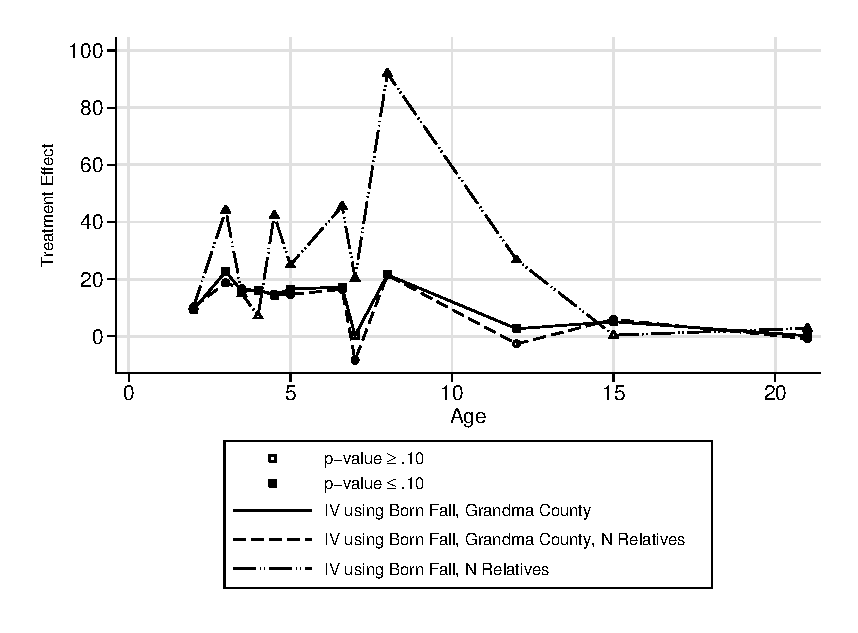
\includegraphics[width=.8\columnwidth]{output/appendixplots/ins_inter_logQ_iv_te.eps}
\floatfoot{
\footnotesize
\noindent Note: This plot presents the parameter associated with $D$ estimated using Control Functions as described in the text. The outcomes ($Y$) are IQ scores at different ages with a national standard deviation of 15 and a mean of 100.  $D=1$ for subjects that participate in ABC/CARE center-based childcare, and $D=0$ for subjects who do not participate in treatment. $Q$ is the number of months attending preschool. It is coded as zero for subjects participating in ABC/CARE. $\mathbf{X}$ includes a set of controls selected from all available baseline controls to maximize explanatory power across all outcomes tested in the paper: gender of the subject, mother's IQ score, High-risk Index, and Apgar Score at 1 minute.}
\end{figure}

\begin{figure}[H]
		\caption{Effect of Center-based Childcare on Labor Market Outcomes, Accounting for Endogenous (log) Months of Take-up of Alternative Preschool} \label{output/appendixplots/Q_cf_te.eps}
		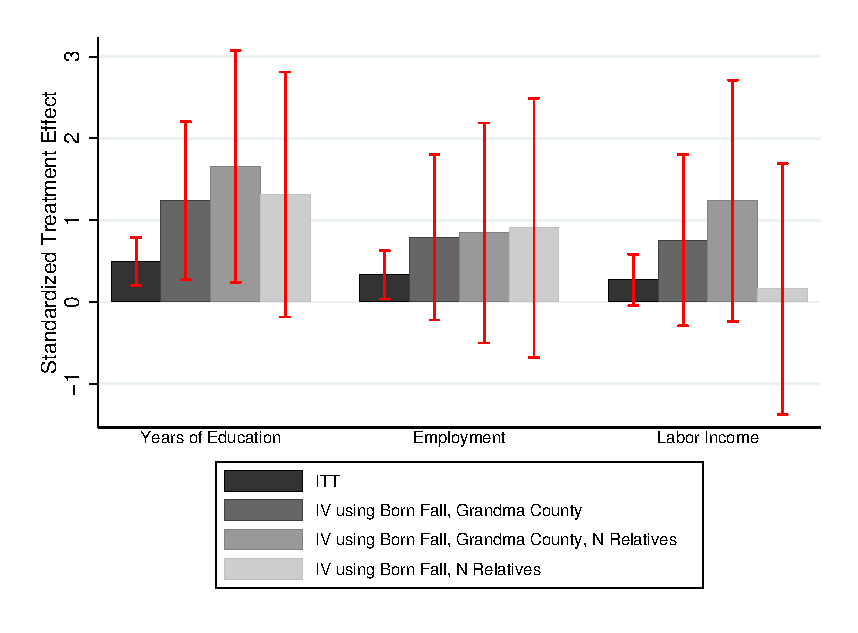
\includegraphics[width=.8\columnwidth]{output/appendixplots/ins_inter_logQ_iv_other.eps}
\floatfoot{
\footnotesize
\noindent Note: This plot presents the parameter associated with $D$ estimated using Control Functions as described in the text. The outcomes ($Y$) are different adult outcomes labeled in the horizontal axis.  $D=1$ for subjects that participate in ABC/CARE center-based childcare, and $D=0$ for subjects who do not participate in treatment. $Q$ is the number of months attending preschool. It is coded as zero for subjects participating in ABC/CARE. $\mathbf{X}$ includes a set of controls selected from all available baseline controls to maximize explanatory power across all outcomes tested in the paper: gender of the subject, mother's IQ score, High-risk Index, and Apgar Score at 1 minute.}
\end{figure}